\documentclass[conference]{IEEEtran}


\usepackage[latin1]{inputenc}
\usepackage{hyperref}
\usepackage{amsmath}
\usepackage{amssymb}
\usepackage{color}
\usepackage{amsfonts}
\usepackage{mathtools}
\usepackage{algorithm2e}
\usepackage{graphicx}
\usepackage{fixme}
\usepackage{tikz}
\usepackage{pgfplots}
\usepackage{xcolor}
\usepackage[justification=centering]{caption}
\usepackage{flexisym}
\newcommand\TODO[1]{\textcolor{red}{#1}}
\pgfplotsset{compat=1.9}
\usetikzlibrary{arrows}
\usetikzlibrary{positioning,calc}
\usetikzlibrary{decorations.pathreplacing}
\usetikzlibrary{decorations.markings}
\usetikzlibrary{fit}
\usetikzlibrary{shapes.callouts}
\usetikzlibrary{shapes.geometric}
\usetikzlibrary{matrix}
\usetikzlibrary{spy}

\newcommand{\norm}[1]{\left\lVert #1 \right\rVert}
\def\doubleunderline#1{\underline{\underline{#1}}}
\renewcommand{\vec}[1]{\boldsymbol{#1}}
\newcommand{\p}[1]{\left(#1\right)}
\newcommand{\f}[2]{\frac{#1}{#2}}
\newcommand{\de}[1]{\begin{vmatrix}#1\end{vmatrix}}
\newcommand{\m}[1]{\begin{pmatrix}#1\end{pmatrix}}
\newcommand{\ub}[1]{\underbrace{#1}}
\newcommand{\ubt}[2]{$\underbrace{\mbox{#1}}_{\mbox{#2}}$}
\newcommand{\comb}[2]{{#1 \choose #2}}
\newcommand{\Z}{{\mathbb{Z}}}
\newcommand{\Q}{{\mathbb{Q}}}
\newcommand{\R}{{\mathbb{R}}}
\newcommand{\C}{{\mathbb{C}}}
\newcommand{\N}{{\mathbb{N}}}
\newcommand{\wC}{{\textit{C}}}
\newcommand{\n}{\vskip 6pt \noindent}
\newcommand{\e}{\epsilon}
\newcommand{\notdv}{\thinspace \not | \thickspace}
\newcommand{\union}{\cup}
\newcommand{\inter}{\cap}
\newcommand{\into}{\rightarrow}
\newcommand{\nset}[1]{#1_1,\ldots,#1_n}
\newcommand{\setk}[2]{#1_1,\ldots,#1_#2}
\newcommand{\bnset}[1]{\{#1_1,\ldots,#1_n\}}
\newcommand{\bset}[2]{\{#1_1,\ldots,#1_#2\}}
\newcommand{\ton}[1]{#1=1,\ldots,n}
\newcommand{\tok}[2]{#1=1,\ldots,#2}
\newcommand{\disc}{\operatorname{disc}}
\newcommand{\spn}{\operatorname{Span}}
\newcommand{\rank}{\operatorname{rank}}
\newcommand{\proj}{\operatorname{proj}}
\newcommand{\prp}{\operatorname{perp}}
\newcommand{\ux}{\underline{x}}
\newcommand{\ua}{\underline{a}}
\newcommand{\uu}{\underline{u}}
\newcommand{\pfx}{\frac{\partial f}{\partial x}}
\newcommand{\pfy}{\frac{\partial f}{\partial y}}
\newcommand{\px}{\frac{\partial}{\partial x}}
\newcommand{\pxn}[1]{\frac{\partial f}{\partial x_{#1}}}
\newcommand{\py}{\frac{\partial}{\partial y}}
\newcommand{\jacu}{\frac{\partial(u,v)}{\partial(x,y)}}
\newcommand{\jacx}{\frac{\partial(x,y)}{\partial(u,v)}}
\newcommand{\vzero}{\vec{0}}
\newcommand{\va}{\vec{a}}
\newcommand{\vb}{\vec{b}}
\newcommand{\vc}{\vec{c}}
\newcommand{\vd}{\vec{d}}
\newcommand{\ve}{\vec{e}}
\newcommand{\vh}{\vec{h}}
\newcommand{\vn}{\vec{n}}
\newcommand{\vs}{\vec{s}}
\newcommand{\vu}{\vec{u}}
\newcommand{\vv}{{\vec{v}}}
\newcommand{\vw}{\vec{w}}
\newcommand{\vx}{\vec{x}}
\newcommand{\vy}{\vec{y}}
\newcommand{\vz}{\vec{z}}
\newcommand*{\everymodeprime}{\ensuremath{\prime}}
\begin{document}

\title{Neural Machine Translation}
\vspace{-1.5cm}
\author{\IEEEauthorblockN{Seminar Report-NLP}
\IEEEauthorblockN{Arul, Ehsan}
\IEEEauthorblockA{Rheinische Friedrich-Wilhelms-Universit\"at Bonn}
\IEEEauthorblockA{\today}
}

\maketitle


\begin{abstract}
Abstract

\end{abstract}


\section{Introduction}


\section{Deep Learning - An Introduction}

In the recent  years, Deep learning has been making a big impact in various fields of computer science. This impact is profound in the perceptual learning task in the fields like computer vision, natural language processing, etc, \cite{lecun2015deep}. Though the idea of training a multi layered neural network to perform function approximation is known to the research community for at least a couple of decades\cite{schmidhuber2015deep}, due to the nature of training problem requiring large computational resources, the multi layered neural network remained less practical. With the advent of general purpose graphical processing units(GPGPUs) and the availability of training data, the neural networks are now a practical solution for many perceptual tasks. One of the early success of deep learning was in the field of image classification. In the annual ImageNet classification challenge \cite{deng2009imagenet}, AlexNet \cite{krizhevsky2012imagenet} showed a remarkable improvement in the state-of-the-art accuracy. Within a few years, more sophisticated architectures like Google Inception Network \cite{szegedy2016rethinking}, Deep Residual Network \cite{he2016deep}, etc., has improved the accuracy to be comparable with a human in that task. The generality of the neural network made it easily possible to be used for a wide variety of tasks. With more people working on deep learning and the ideas arising in solving on the problems being easily transferable, the deep learning is the state-of-the-art for many learning tasks. In the following section, we will briefly summarize the basics of deep learning.


The basic building block of a Multilayer network, or in more technical term Multilayer  perceptron(MLP) is a perceptron. The preceptron \ref{fig:ann} closely resembles a neuron in a human brain \ref{fig:neuron}. A preceptron takes a set of input values, computes a weighted sum of the inputs, and outputs a scalar value of a after applying an activation function (mostly non-linear). The weights for computing the weighted sum and the threshold in the activation function are initially set to random values and are learned from the training data. 
Mathematically, a perceptron with the weight matrix $A$ and the threshold $T$ for an step activation function, for the input vector $x$, outputs the following,


\[
    f(x)= 
\begin{cases}
    1,& \text{if }  A x > c \\
    0,              & \text{otherwise}
\end{cases}
\]

A layer has many number of neurons and many layers are stacked one on top of the other to form a MLP. An MLP with very many layers is called as Deep Neural Network(DNN). In the following section we will discuss the properties of DNNs and how they are useful in the context of supervised machine learning.


\begin{figure}
    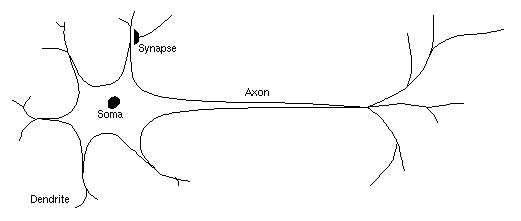
\includegraphics[width=.99\linewidth]{img/bioneuron.jpg}  
    \caption{A biological neuron.}
    \label{fig:neuron}
\end{figure}

\begin{figure}
    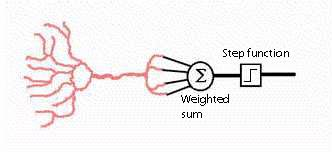
\includegraphics[width=.99\linewidth]{img/artificial.jpg}  
    \caption{ An artificial neuron (perceptron)}
    \label{fig:ann}
\end{figure}


\begin{figure}
    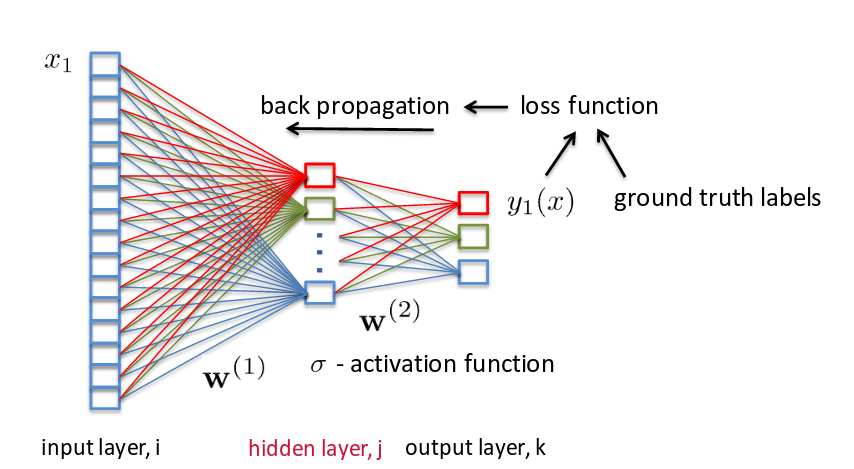
\includegraphics[width=.99\linewidth]{img/mlp.png}  
    \caption{Layered representation in an MLP}
    \label{fig:ann}
\end{figure}


\subsection{Supervised learning}
Supervised learning is the problem of predicting an new output $y\everymodeprime$  for a new input $x\everymodeprime$, and set of training data that provides a set of input and output $\{x \mapsto y\}$. Most of the supervised learning problems can be formulated as either a classification or regression problem. Classification is the problem of predicting the label for a given  $x\everymodeprime$ among a set of given labels $\{Y\}$ while regression of predicting a continuous  valued output for a given input. The usual way of doing supervised learning is to extract features from the given data and train a model to perform classification or regression. 


$$x \xrightarrow[\text{Feature extraction}]{ \mathbb{D}(x) } x\everymodeprime _{intermediate} \xrightarrow[\text{classifer/regressor}]{\mathbb{F}(x\everymodeprime | \theta)}   y$$

The power of the DNNs lie in the fact that the models learns the features directly from the given training data and avoids hand engineered features. 
$$ x \xrightarrow[ \text{hierachical}] { \mathbb{M}(x | \Theta) } y$$
\bibliographystyle{plain}

The DNNs with neurons in one layers being connected to all the neurons in the next layer are called Feed Forward Networks. The feed forward networks are harder to train since they have lots of parameters. To make a the DNNs learn useful representation for performing supervised learning, we need special types of connections between the neurons. Two of the most commonly used DNN architectures are Convolutional Neural Networks(CNN) and Recurrent Neural Networks(RNN). In the following section we will discuss these architectures in detail.


\bibliography{literature}
\end{document}



